\section{Analisi statistica Jabref}

\subsection{Analisi Statistica Technical Debt}
In \autoref{td-tipo} è possibile osservare la dimensione del technical debt rispetto alla tipologia di clone. L'analisi statistica è confermata dal p-value, ottenuto con il test di Kruskal-Wallis mediante R, che ha un valore inferiore a $2,2 e^{-16}$.
\begin{figure}[htbp]
	\centering
	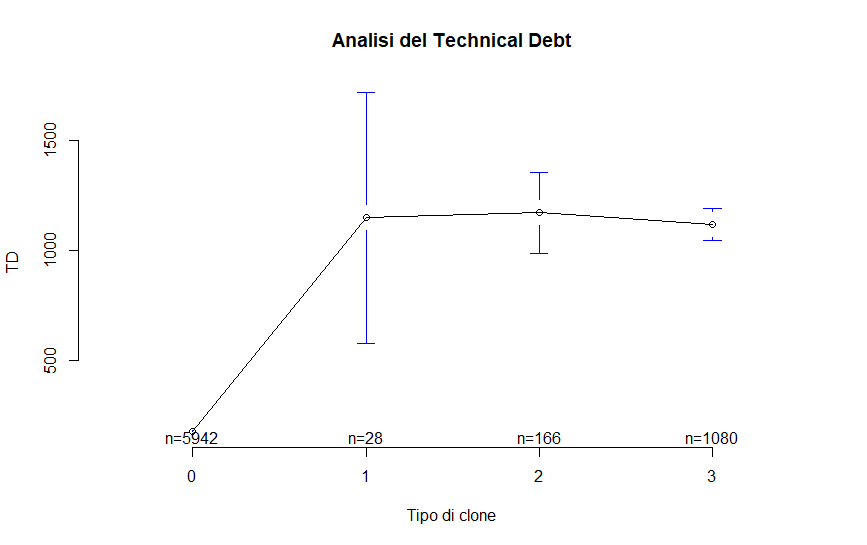
\includegraphics[scale=0.5]{analisi_R/AnalisiJabref/1-gplot-td-type.png}
\caption{Analisi statistica Technical Debt JabRef}
\label{td-tipo}
\end{figure}

Il grafico in \autoref{td-tipo} presenta sull'asse delle ascisse il tipo di clone, indicando con zero le classi in cui il codice clonato è assente. Si riporta, invece, sull'asse delle ordinate il valore del technical debt. Si indica con n il numero delle occorrenze dei cloni di ciascun tipo presenti nelle quattro versioni del progetto. Essendo un'analisi statistica, si rapporta il technical debt totale al numero di occorrenze complessive. Di conseguenza, essendo il numero di cloni di tipo 3 molto maggiore rispetto a quello dei cloni di tipo 1, il technical debt medio risulta minore per i cloni di tipo 3. Questo risultato potrebbe apparentemente confutare quanto sostenute precedentemente, ossia che per i cloni di tipo 3 il technical debt è maggiore. In realtà non è così in quanto, nell'analisi statistica, si tiene conto del numero totale di occorrenze.

\subsection{Analisi Statistica Code Smells}
In \autoref{codesmell-tipo} si mostra la quantità di code smells rispetto alla tipologia di clone. Questa analisi statistica è confermata dal p-value, ottenuto con il test di Kruskal-Wallis mediante R, che ha un valore inferiore a $2,2 e^{-16}$.
\begin{figure}[htbp]
	\centering
	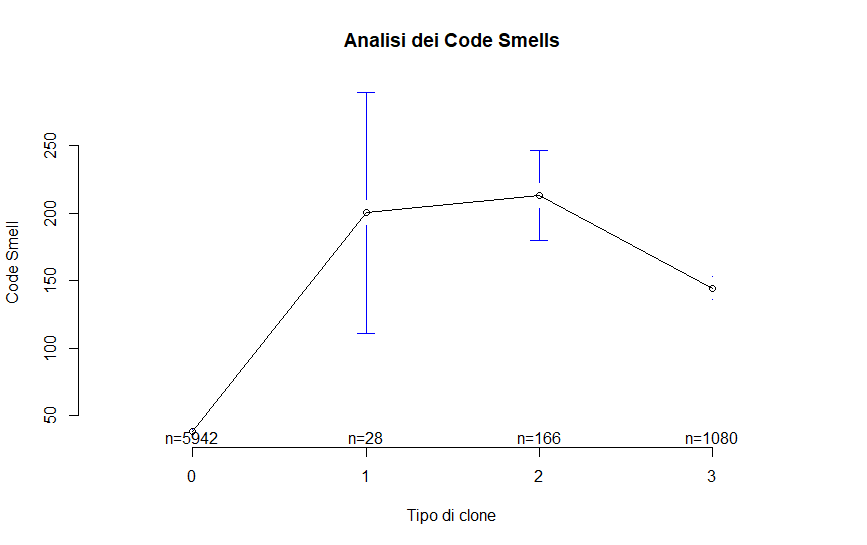
\includegraphics[scale=0.5]{analisi_R/AnalisiJabref/2-gplot-codesmell-type.png}
\caption{Analisi statistica Code Smell JabRef}
\label{codesmell-tipo}
\end{figure}

Il grafico in \autoref{td-tipo} presenta sull'asse delle ascisse il tipo di clone, indicando con zero le classi in cui il codice clonato è assente. Si riporta, invece, sull'asse delle ordinate il numero di code smells. Si indica con n il numero delle occorrenze dei cloni di ciascun tipo presenti nelle quattro versioni del progetto. Le considerazioni risultano analoghe al caso precedente, concludendo che l'analisi statistica non confuta i risultati ottenuti in precedenza.

\subsection{Analisi Statistica Lunghezza Codice Clonato}
In \autoref{len-tipo} si mostra la lunghezza del codice clonato (espressa in LOC) rispetto alla tipologia di clone. Questa analisi statistica è confermata dal p-value, ottenuto con il test di Kruskal-Wallis mediante R, che ha un valore inferiore a $2,2 e^{-16}$. \newpage
\begin{figure}[htbp]
	\centering
	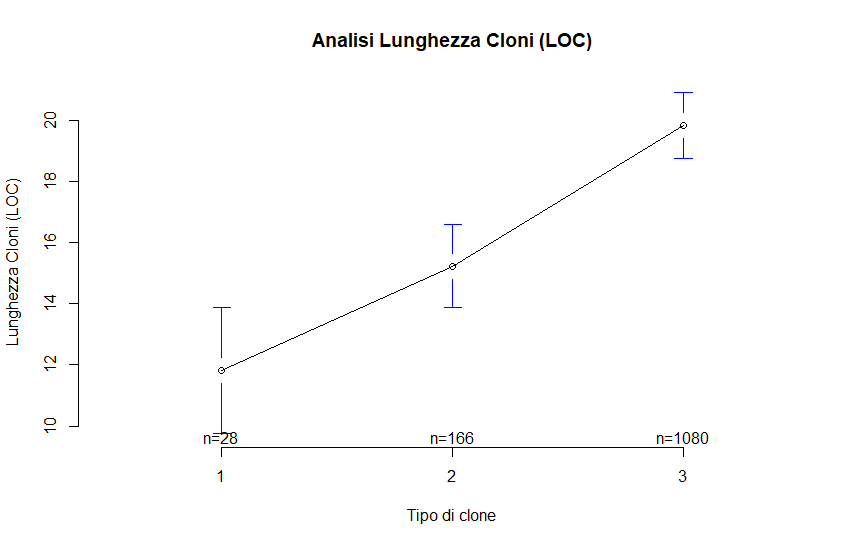
\includegraphics[scale=0.5]{analisi_R/AnalisiJabref/3-gplot-len-type.png}
\caption{Analisi statistica Lunghezza Codice Clonato JabRef}
\label{len-tipo}
\end{figure}

In \autoref{len-tipo} si riporta sull'asse delle ascisse il tipo di clone e sull'asse delle ordinate il numero di LOC. Si nota che i cloni di tipo 3 hanno in media numero di LOC maggiore rispetto ai cloni di tipo 1 e 2.
